\newpage
\subsection{Exponentialfunktionen}


allgemeine Form: $y=a^x$
\begin{itemize}
    \item wenn $a>1$: Wachstum der Funktion
    \item wenn $0<a<1$: Zerfall der Funktion
\end{itemize}

\hfill \break
Eigenschaften:
\begin{itemize}
    \item alle Funktionen vom Typ $y=a^x$ haben den Punkt $P(0|1)$ gemein.
    \item alle Funktionen vom Typ $y=a^x$ gehen durch den Punkt $P(1|a)$, da $y=a^1 = a$.
    \item $y=a^x$ ist zu $y=a^{-x}$ symetrisch bezüglich der y Achse.
    \item die Funktion $y=a^x$ kann nie negativ werden also hat sie keine Nullstellen.
    \item Die x Achse ist eine Asymptote da die Funktion 0 niemals berührt.
\end{itemize}

\hfill \break
Die Wertetabellen und Grafik für \textcolor{red}{$y=2^x$} und \textcolor{blue}{$y=2^{-x}$}:\\

\hfill \break
\fboxrule=0.8pt \fcolorbox{lightgray}{lightgray}{%
    \begin{tabular}{c|c||c|c}
        \textcolor{red}{$x$} & $y$  & \textcolor{blue}{$x$} & $y$  \\
        \hline
        -2                   & 0.25 & -2                   & 4    \\
        -1                   & 0.5  & -1                   & 2    \\
        0                    & 1    & 0                    & 1    \\
        1                    & 2    & 1                    & 0.5  \\
        2                    & 4    & 2                    & 0.25 \\
    \end{tabular}}

\hfill \break
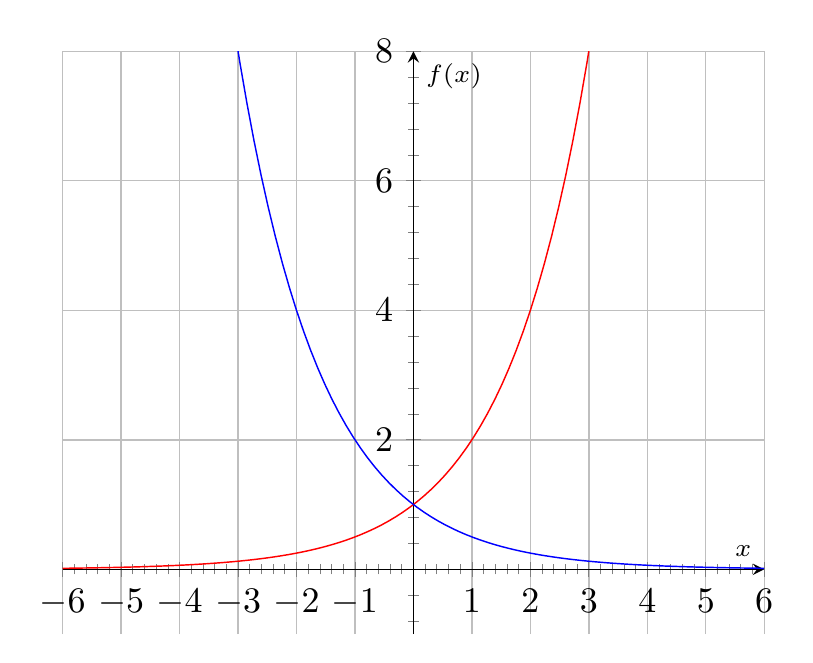
\begin{tikzpicture}[scale=1.3]
    \begin{axis}%
        [
            grid=major,
            xtick={-7,-6,...,7},
            minor x tick num=4, % 4 minor ticks => 5 subintervals
            xmin=-6,
            xmax=6,
            xlabel={\scriptsize $x$},
            axis x line=middle,
            ytick={-1,-5,...,7},
            minor y tick num=4,  % 4 minor ticks => 5 subintervals
            ymin=-1,
            ymax=8,
            ylabel={\scriptsize $f(x)$},
            axis y line=middle,
            no markers,
            samples=100,
            domain=-6:6,
        ]
        \addplot[red] (x,{2^x});
        \addplot[blue] (x,{2^-x});
    \end{axis}
\end{tikzpicture}